\documentclass[11pt,a4paper]{article}

\usepackage{style2017}
\usepackage{hyperref}

\hypersetup{
    colorlinks =false,
    linkcolor=blue,
   linkbordercolor = 1 0 0
}
\newcounter{numexo}
\setcellgapes{1pt}

\begin{document}



\begin{NSI}
{Exercice}{Encodage des caractères}
\end{NSI}


\addtocounter{numexo}{1}
\subsection*{\Large Exercice \thenumexo }
On redonne la table ASCII:
\begin{center}
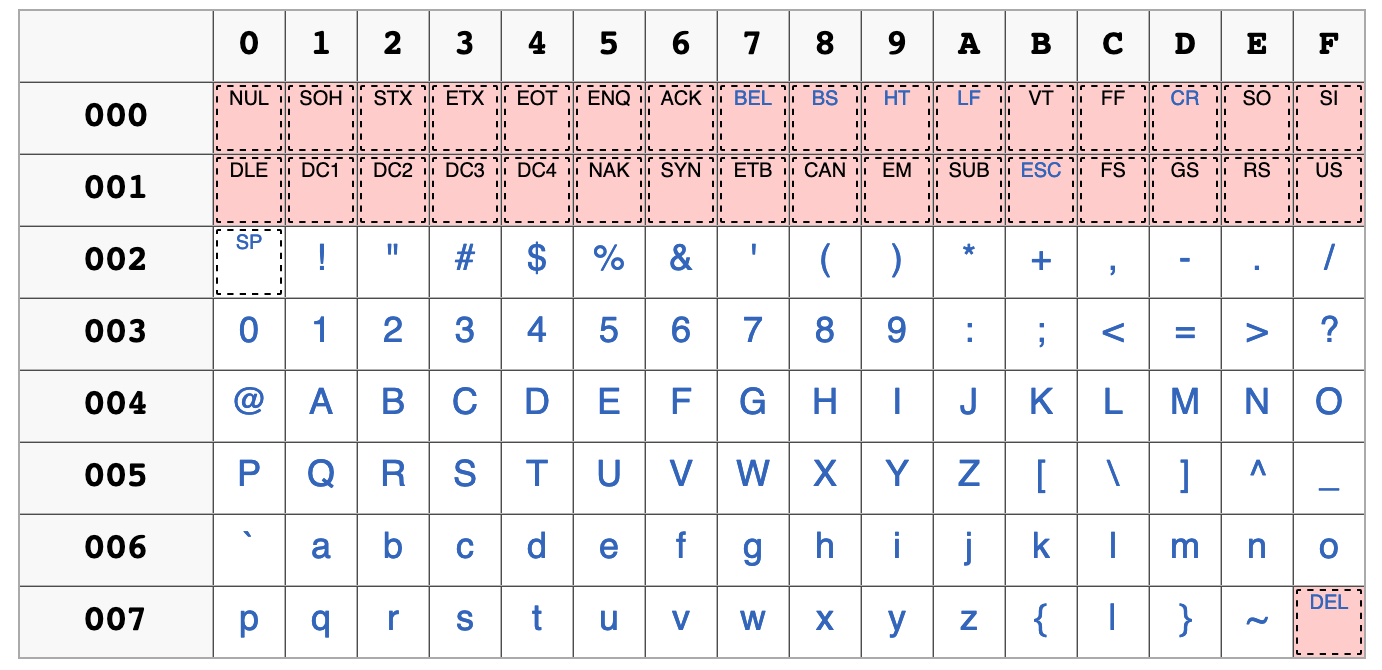
\includegraphics[scale=0.5]{tableASCII.png}
\end{center}
\begin{enumerate}
\item Que remarque-t-on dans la table ASCII en observant les lettres majuscules et les lettres minuscules ?
\item Donner les codes binaires des lettres A, a, M, m et W, w.
\item Quelle observation peut-on faire entre le codage binaire des majuscules et celui des minuscules?
\end{enumerate}

\addtocounter{numexo}{1}
\subsection*{\Large Exercice \thenumexo }
\begin{enumerate}
\item Ouvrir le bloc-note de windows puis taper la phrase "Les élèves à l'école."
\item Enregistrer le fichier avec l'extension txt.
\item Ouvrez votre fichier avec Libre office. Que remarquez-vous ?
\item Quelle explication peut-on donner ?
\item Télécharger le fichier html ex-encodage-utf-iso-html.html, l'ouvrir avec votre navigateur puis répondre aux questions.
\end{enumerate}


\addtocounter{numexo}{1}
\subsection*{\Large Exercice \thenumexo }
Dans la langue française, on retrouve des ligatures, c'est à dire que certaines lettres sont collées l'une à l'autre. Par exemple, le o et le e sont collés dans les mots n{\oe}ud, {\oe}il et {\oe}uvre.

La ligature \oe ~est apparue dans la table ISO 8859-15 avec le code hexadécimal $BD$.

Dans la norme Unicode, cette ligature a pour point de code \textbf{U+0153}.

On rappelle que le codage binaire en UTF-8 se fait en suivant les indications du tableau ci-dessous.
\begin{center}
\begin{tabular}{|C{4cm}|L{8cm}|L{2cm}|}\hline
Plage & Suite d'octets (en binaire) & bits codant\\\hline
U+0000 à U+007F & $0xxx xxxx$ & 7 bits\\
U+0080 à U+07FF & $110x xxxx$ $10xx xxxx$ & 11 bits\\
U+0800 à U+FFFF & $1110 xxxx$ $10xx xxxx$ $10xx xxxx$ & 16 bits\\
U+10000 à U+10FFFF & $1111 0xxx$ $10xx xxxx$ $10xx xxxx$ $10xx xxxx$ & 21 bits\\\hline
\end{tabular}
\end{center}

\begin{enumerate}
\item Donner, selon la norme ISO, le codage binaire de la ligature \oe.
\item Combien faut-il d'octets pour coder la ligature {\oe} en UTF-8
\item Après avoir converti le point de code en binaire, en déduire le codage binaire en UTF-8 de la ligature {\oe}.
\end{enumerate}

\end{document}

